%\thispagestyle{myheadings}
\newpage
\section{Keynote Speaker}
\index{Coulson, Seana}

\begin{center}
{\bfseries\Large Distributional Semantics:\\\vspace{2.0\lineskip}What do large language models have to say?} \\
\vspace{1.0em}
{\large\bf Seana Coulson} \\
University of California, San Diego

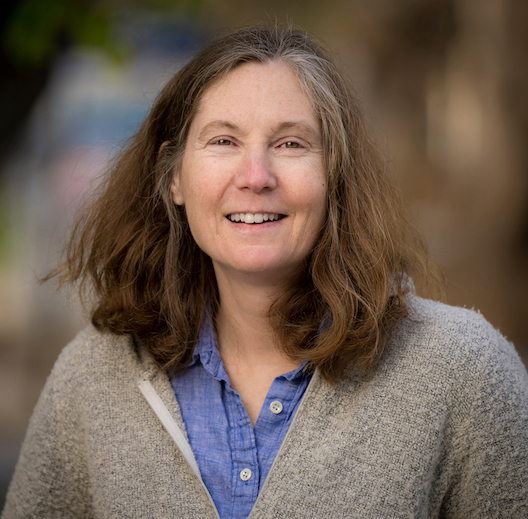
\includegraphics[width=0.4\linewidth]{content/day3/seana-headshot.png}

\textbf{\daydateyear{}, 14:00--15:00 CST}\\
\textbf{\PlenaryLoc{}}
\end{center}

\noindent
{\bfseries Abstract:} 
Large language models motivate an approach to meaning known as distributional semantics, that words mean what they do because of how they're distributed in language. In this talk I will describe some evidence from my lab that suggests metrics from large language models do a good job of predicting behavioral and neural responses to some aspects of human language. I go on to describe some research that highlights important differences in meaning processing in humans and the `understanding' displayed by language models. Discrepancies are particularly noteworthy in studies of joke comprehension.

\vspace{1em}

{\bfseries Biography:} 
Seana Coulson received her Ph.D.~in Cognitive Science from the University of California San Diego in 1997. The recipient of fellowships from the McDonnell Pew foundation and the NIH NRSA, she worked as a post-doctoral fellow in the Psychology Department at the University of Arizona from 1997--1999. In 1999, she returned as faculty to UC San Diego's Cognitive Science Department. She is currently a full Professor, holds the Jeffrey Elman Chancellor's Endowed Chair of Cognitive Science, and co-directs the UCSD/SDSU Joint Doctoral Program in Language and Communicative Disorders. She directs the Brain and Cognition Lab at UC San Diego where her research concerns how people understand language and other meaningful stimuli.

\newpage
